\documentclass[conference]{IEEEtran}
% \IEEEoverridecommandlockouts
% The preceding line is only needed to identify funding in the first footnote. If that is unneeded, please comment it out.
\usepackage{cite}
\usepackage{amsmath,amssymb,amsfonts}
\usepackage{graphicx}
\usepackage{textcomp}
\usepackage{xcolor}
\usepackage{booktabs}
\usepackage{tabularx}
\usepackage{makecell}
\usepackage{url}
\usepackage{tikz}
\usetikzlibrary{shapes.geometric, arrows.meta, positioning}
\def\BibTeX{{\rm B\kern-.05em{\sc i\kern-.025em b}\kern-.08em
    T\kern-.1667em\lower.7ex\hbox{E}\kern-.125emX}}
\begin{document}
\raggedbottom

\title{Speech-Native Retrieval-Augmented Generation for Agricultural Advisory in Low-Resource Dialects \\
% {\footnotesize \textsuperscript{*}Note: Sub-titles are not captured in Xplore and
% should not be used}
% \thanks{Identify applicable funding agency here. If none, delete this.}
}
% Identify applicable funding agency here. If none, delete this.

\author{\IEEEauthorblockN{Darshan Pundlik Heble}
\IEEEauthorblockA{\textit{PG Scholar, Department of Computer Science} \\
\textit{Christ (Deemed to be University)}\\
Bangalore, India \\
darshanpundlik.heble@mca.christuniversity.in }
% \and
% \IEEEauthorblockN{2\textsuperscript{nd} Given Name Surname}
% \IEEEauthorblockA{\textit{dept. name of organization (of Aff.)} \\
% \textit{name of organization (of Aff.)}\\
% City, Country \\
% email address or ORCID}

}

\maketitle

\begin{abstract}
Smallholder farmers in low-literacy, dialect-rich regions face a persistent barrier to digital agricultural advisory: existing voice-enabled systems rely on a cascaded pipeline in which automatic speech recognition (ASR) first transcribes a spoken query before retrieval-augmented generation (RAG) produces an answer. Because domain-critical terminology — pesticide names, crop diseases, and pest names — is disproportionately subject to ASR substitution errors, and because farmers frequently use dialect-specific or colloquial terms absent from standard ASR training data, transcription errors propagate directly into retrieval failures and, ultimately, into incorrect agricultural advice. Recent work has shown that retrieval can be performed directly on speech embeddings without an intermediate transcription step, removing one source of cascade error; however, no existing system addresses the compounding effect of dialect variation and domain-critical rare vocabulary together, nor combines speech-native retrieval with an explicit dialect-to-scientific-entity mapping layer, confidence-gated escalation to a human expert, and fully offline operation on resource-constrained hardware. This paper proposes a framework that integrates these four components and outlines an experimental protocol — comparing ASR-cascaded, keyword-based, dense semantic, and hybrid retrieval under dialect variation — to evaluate whether this combination improves retrieval accuracy and answer reliability for agricultural advisory in low-resource dialect settings. A runnable software prototype of the proposed pipeline was built and measured end to end on small, demo-scale data as a preliminary mechanism check: it confirms that dialect mapping is what makes dialectal queries retrievable at all in this setting and that per-stage latency fits comfortably within a consumer 6~GB-VRAM budget, while also surfacing two open problems — a speech-native retrieval adapter that does not yet generalize past its training distribution, and a confidence-gate signal whose validation revealed it was less discriminative than intended — that remain unresolved pending evaluation on real target-dialect speech, which does not yet exist.
\end{abstract}

\renewcommand\IEEEkeywordsname{Keywords}
\begin{IEEEkeywords}
Agricultural advisory systems, dialect-aware retrieval, low-resource languages, speech-native RAG.
\end{IEEEkeywords}

\section{Introduction}
Agricultural extension — the transfer of evidence-based farming knowledge to smallholder farmers — remains a critical bottleneck in regions with low literacy and limited connectivity. RAG-based advisory systems such as Farmer.Chat \cite{farmerchat2024} and KrishokBondhu \cite{ameen2026krishokbondhu} show that voice-enabled, multilingual chatbots can reduce farmers' dependence on scarce extension agents, and systems such as SukhaRakshak AI \cite{iwmi2025sukharakshak} extend this to more than twenty Indian languages. All of them, however, first transcribe a spoken query via automatic speech recognition (ASR) before retrieval proceeds on the resulting text — a cascaded design vulnerable to a specific failure mode. ASR errors on Indian-language agricultural speech disproportionately affect domain-critical terms such as crop, chemical, and pest names \cite{benchmarkingasr2026}, and this degrades further under dialectal and code-mixed variation \cite{dialectmatters2026}. A mistranscribed pest or disease term propagates directly into retrieval, surfacing an irrelevant document and ultimately an incorrect recommendation.

One way to remove this failure mode is to retrieve directly from a speech representation, bypassing transcription entirely — a direction that has recently moved from proposal to validated, production-deployed technique. Amazon's SpeechRAG \cite{min2025speechrag} aligns a speech encoder with a frozen text-retrieval embedding space to retrieve audio passages without ASR, and Google's Speech-to-Retrieval (S2R) \cite{google2025s2r} performs an analogous mapping live in production for Voice Search. Neither system, however, has been evaluated under dialect variation or domain-critical rare-entity retrieval such as pesticide and pest names, and neither normalizes the many regional or colloquial terms a farmer may use for the same concept. Existing agricultural knowledge graphs \cite{wu2026cropgraphrag, kgeditorial2023} normalize only standardized, written terminology, leaving vernacular-to-scientific mapping for spoken queries an open problem.

A further limitation is that existing systems answer regardless of confidence, even though incorrect agricultural advice can damage a season's crop — an argument made explicitly for comparably high-stakes RAG deployments in clinical and financial domains \cite{dependablerag2026, abstinence2025}, though naive confidence signals are known to misfire in both directions \cite{intrygue2026} and require validation rather than blind trust. Most RAG research also implicitly assumes reliable connectivity and cloud-hosted inference \cite{compactllm2026}, which the rural settings these systems target frequently lack. Taken together, no existing system combines speech-native retrieval, dialect-to-entity mapping, confidence-gated escalation, and offline operation for agricultural advisory in low-resource dialects. This paper addresses that combination and poses the following research questions:

\begin{itemize}
    \item \textbf{RQ1:} Does speech-native retrieval retain its advantage over ASR-cascaded retrieval under dialect variation and domain-critical rare vocabulary?

    \item \textbf{RQ2:} Does a dialect-to-scientific-entity mapping layer improve retrieval accuracy for queries phrased in regional or colloquial terms?

    \item \textbf{RQ3:} Can the pipeline operate fully offline, on resource-constrained consumer hardware, at acceptable latency and accuracy?

    \item \textbf{RQ4:} Does hybrid (lexical + dense) retrieval combined with dialect mapping outperform either method alone on queries containing domain-critical rare entities?
\end{itemize}

The main contributions of this paper are:


\begin{itemize}
    \item Identifying a specific, underaddressed gap in speech-native agricultural retrieval---dialect variation combined with domain-critical rare vocabulary---not addressed by existing speech-native retrieval systems \cite{min2025speechrag, google2025s2r}.

    \item A dialect-to-scientific-entity mapping layer bootstrapped from low-cost, publicly available resources rather than new dialect speech collection.

    \item A confidence-gated RAG architecture that escalates low-confidence queries to a human expert.

    \item A system design and experimental protocol scoped to consumer-grade, GPU-constrained hardware, reserving cloud GPU resources only for one-time adapter training.
\end{itemize}


The remainder of this paper is organized as follows: Section II reviews related work; Section III presents the proposed architecture; Section IV describes the experimental protocol designed to evaluate it; Section V outlines the evaluation plan and expected outcomes for each research question, since that protocol has not yet been executed on the target dialect; Section VI reports real, measured preliminary results from a runnable software prototype of the architecture on demo-scale data, distinct from Section V's still-open hypotheses; and Section VII concludes.

\section{Literature Review}

% \subsection{Maintaining the Integrity of the Specifications}

\subsection{AI-Driven Agricultural Advisory Systems}

A growing body of work applies retrieval-augmented generation to agricultural advisory. Farmer.Chat \cite{farmerchat2024} is the most widely cited system, deployed across Kenya, India, Ethiopia, and Nigeria and engaging over 15,000 farmers across more than 300,000 queries; it supports more than 40 crops with multilingual, multimodal (text, voice note, image) input, ingesting structured and unstructured sources into a dynamic knowledge base. KrishokBondhu \cite{ameen2026krishokbondhu} is architecturally the closest system to the present proposal: a phone-call-based, fully voice-in/voice-out RAG pipeline for Bengali farmers in which OCR-digitized agricultural handbooks are vectorized, ASR transcribes the call, a vector database retrieves relevant passages, a small language model generates a grounded response, and text-to-speech delivers the answer; in pilot evaluation it produced high-quality answers for 72.7\% of queries and outperformed the KisanQRS benchmark \cite{rehman2023kisanqrs} by 44.7\% on a composite quality score. SukhaRakshak AI \cite{iwmi2025sukharakshak} integrates national language-AI infrastructure to deliver drought advisories in more than twenty Indian languages. AgroLLM \cite{agrollm2025} describes a simpler FAISS-based RAG chatbot for general agricultural question answering.

Three further systems are close enough in scope to merit individual discussion. A.A.H.A.R. \cite{dubey2025aahar} combines an offline, quantized LLM with an ASR component fine-tuned specifically for agricultural vocabulary and regional accents, reporting sub-2-second response times and high user satisfaction in its "Aahar" app; however, it remains a cascaded ASR-then-text architecture — its ASR is adapted to dialects, but retrieval still depends on the resulting transcript, and it includes neither speech-native retrieval nor confidence-gated escalation. Krishi Sathi \cite{vijayvargia2025krishisathi} is an intent-aware, multi-turn agricultural question-answering chatbot with ASR and TTS for accessibility in English and Hindi, reporting 97.53\% query response accuracy and sub-6-second response times, but follows the same ASR-then-retrieval design and does not address dialect variation specifically. A cross-lingual RAG case study for Bengali agricultural advisory \cite{hossain2026bengalirag} is presently text-only and already introduces a keyword-injection strategy to bridge colloquial farmer terminology with scientific nomenclature — a text-domain analog of this paper's proposed dialect-mapping layer — but its own discussion explicitly names ASR integration and dialect-aware normalization of spoken queries as future work it has not yet undertaken, independent confirmation from within the same problem space that this combination remains open.

None of the systems surveyed here treats ASR-induced retrieval failure on dialect-specific or domain-critical terminology as a first-class design problem to be solved by restructuring retrieval; the closest, A.A.H.A.R. and Krishi Sathi, address dialect variation only by adapting the ASR component itself.

\subsection{Speech Processing for Low-Resource Indian Languages and Dialects}

Benchmarking work on ASR for Indian-language agricultural speech \cite{benchmarkingasr2026} finds that standard word error rate (WER) under-penalizes errors on domain-critical terms, proposing an agriculture-weighted metric that shows the dominant ASR confusion pairs across languages involve crop, chemical, and pest or disease vocabulary specifically. A complementary study on cross-lingual ASR transfer for low-resource Indic dialects \cite{dialectmatters2026} quantifies how code-mixing and orthographic variation degrade transcription accuracy for dialect varieties such as Garhwali, building on national speech-data initiatives including Bhashini, Vakyansh, and IndicWav2Vec, and notes that no prior work had trained or evaluated an ASR model for that dialect at all. Dialect-specific speech corpora, such as a 250-hour Chhattisgarhi ASR dataset \cite{singh2023respin} produced under the RESPIN initiative and a dedicated Malayalam agricultural speech corpus, show that domain- and dialect-specific resources exist for some Indian languages but remain incomplete in coverage — most Indian dialects, including the one targeted in this paper, have no comparable resource yet.

\subsection{Speech-Native Retrieval}

SpeechRAG \cite{min2025speechrag} fine-tunes an adapter that projects speech-encoder representations into the embedding space of a frozen text retriever, enabling direct retrieval of audio passages from text or speech queries without an ASR step; retrieval experiments on spoken question-answering benchmarks show this approach matches or exceeds an ASR-then-text-retrieval cascade. Google's S2R \cite{google2025s2r} performs an analogous dual-encoder mapping in a production voice-search system and is accompanied by the Simple Voice Questions benchmark spanning seventeen languages. Underlying both approaches are self-supervised speech representation models such as wav2vec 2.0 \cite{baevski2020wav2vec} and HuBERT \cite{hsu2021hubert}, and the broader "textless NLP" literature \cite{spidr2025}, which has found that representations optimized for ASR accuracy are not necessarily optimal for downstream spoken-language tasks. Multilingual speech-translation foundation models such as SeamlessM4T \cite{barrault2023seamlessm4t} provide an additional source of pretrained multilingual speech encoders relevant to adapter-based approaches. Critically, neither SpeechRAG nor S2R has been evaluated under dialect variation or domain-critical rare-entity retrieval, and neither targets agriculture as an application domain — both are general-purpose systems whose published evaluations use standard, well-resourced language varieties.

\subsection{Retrieval Strategy: Keyword, Dense, and Hybrid Search}

Comparative studies of retrieval strategy \cite{sultania2024hybridsearch} consistently find that dense (semantic) retrieval outperforms lexical retrieval on paraphrased queries with little lexical overlap with the target document, while lexical methods such as BM25 retain an advantage on exact, rare, domain-specific entities — a category that includes pesticide and disease names directly relevant to agricultural queries. Hybrid retrieval, fusing lexical and dense signals, has been shown to outperform either method alone in domain-specific question answering. This is a practically important finding for the present proposal: a naive "speech embeddings beat keywords" framing would risk a result where keyword matching wins precisely on the safety-critical query category (pesticide and pest names), making hybrid retrieval — rather than a strict either/or comparison — the more defensible retrieval backbone.

\subsection{Dialect-Aware and Colloquial-to-Formal Knowledge Representation}

Agricultural knowledge graphs are a mature area of work, almost entirely built from standardized written text. Crop GraphRAG \cite{wu2026cropgraphrag} constructs a multi-relational knowledge graph spanning 28 crop categories, with retrieval performed jointly over graph subgraphs and text passages. The AgCNER dataset \cite{yao2024agcner} supports named-entity recognition for agricultural pests and diseases at scale. At the standards level, the EPPO ontology and related efforts \cite{kgeditorial2023} provide cross-system interoperable codes for plant and pest entities.

Closer to the present proposal's dialect-mapping layer, two recent works address the gap between informal farmer language and formal agricultural terminology — but neither in speech. Liu et al. \cite{liu2025colloquialpest} propose a soft-prompt-tuning method that extracts agricultural entities from colloquial, unstructured symptom descriptions using a pretrained agricultural language model, queries an agricultural knowledge graph for the matched entities, and classifies the pest or disease from the combined representation, reporting that conventional classifiers degrade substantially on farmers' natural, fuzzy language. The Bengali cross-lingual RAG case study \cite{hossain2026bengalirag} takes a simpler approach, injecting domain-specific keywords to bridge colloquial Bengali terms with scientific English nomenclature before retrieval. Both confirm that the colloquial-to-formal mapping problem is real, actively studied, and tractable — but both operate on written text, leaving the speech-domain version of this same mapping problem, applied to retrieval rather than classification, open.

\subsection{Confidence Estimation in RAG}

Dependable RAG work \cite{dependablerag2026} categorizes hallucination detection into closed-book methods, which rely on internal model signals, and open-book methods, which compare model behavior with and without retrieved context. Confidence-gated abstention has been argued for explicitly in high-stakes RAG deployments in clinical decision support and financial advisory, where the cost of a confident wrong answer exceeds the cost of abstaining \cite{abstinence2025}. However, naive entropy-based confidence signals have been shown to misfire in both directions, flagging correct, well-grounded answers as uncertain due to interactions between attention mechanisms and entropy computation \cite{intrygue2026}, indicating that a confidence-gating layer requires validation against labeled correct/incorrect examples rather than being assumed reliable by construction.

\subsection{Offline and Edge Deployment of Language Models}

Quantization and on-device deployment of large language models is an active systems research area. Reported figures for 4-bit quantized Llama-3 8B indicate usable but slow inference (2–3 tokens/second) on smartphones with at least 6 GB of RAM, with 8-bit variants requiring a discrete GPU with at least 8 GB of VRAM for comparable throughput \cite{compactllm2026}. Within agriculture specifically, A.A.H.A.R. \cite{dubey2025aahar} and the Bengali cross-lingual RAG case study \cite{hossain2026bengalirag} both report fully local, consumer-hardware deployments with sub-20-second end-to-end latency, demonstrating that offline agricultural RAG is already practically achievable for text-based systems; whether this holds once a speech-native retrieval and dialect-mapping layer are added is one of this paper's open questions (RQ3). A recent offline plant-disease detection system deployed in rural Tigray \cite{tigray2025plantdisease} demonstrates the broader deployment pattern — quantization, on-device runtime conversion, and dialect-localized interfaces — though for a vision rather than a speech modality.

\subsection{Synthesis}

Taken together, the systems reviewed above each address a subset of the requirements motivated in Section I, but none addresses all of them jointly. Farmer.Chat, KrishokBondhu, SukhaRakshak AI, A.A.H.A.R., and Krishi Sathi demonstrate that voice-enabled agricultural RAG is deployable at scale, but all rely on an ASR-then-retrieval cascade; A.A.H.A.R. and Krishi Sathi only adapt the ASR component to dialects rather than removing the dependence on transcription. SpeechRAG and S2R demonstrate that speech-native retrieval is viable and can outperform the cascade, but neither has been evaluated under dialect variation or domain-critical rare vocabulary, and neither targets agriculture. The colloquial-to-formal mapping work of Liu et al. and the Bengali RAG case study show that normalizing informal terminology is both necessary and actively studied, but only in text. Confidence-gated abstention and offline deployment are each independently established techniques, including within agricultural RAG specifically. The combination of all four — speech-native, dialect-aware, confidence-gated, offline agricultural retrieval — does not appear in any system located during this review, and one of the closest text-based systems in the same problem space explicitly names this combination as unaddressed future work of its own \cite{hossain2026bengalirag}.


\section{Proposed Architecture}

\subsection{Design Overview}

The architecture proposed here integrates the four components motivated in Section I into a single pipeline, illustrated in Fig.~\ref{fig:architecture}. A spoken farmer query is first mapped directly into a retrieval-ready representation without an intervening transcription step (Section III-B); the resulting representation is normalized against a dialect-to-scientific-entity mapping layer so that regional and colloquial terms resolve to the same retrieval targets as their standardized equivalents (Section III-C); retrieval itself is performed by a hybrid lexical-dense retriever, chosen specifically because neither method alone is reliable across both paraphrased and rare-entity queries (Section III-D); the retrieved evidence and a confidence score are then passed through a gate that either proceeds to answer generation or escalates the query to a human expert (Section III-E); and every stage except one-time adapter training is required to execute fully offline on consumer-grade hardware (Section III-F). Each subsection below states the design decision, the prior work it builds on, and the specific gap in that prior work the decision is intended to close.

\begin{figure}[t]
\centering
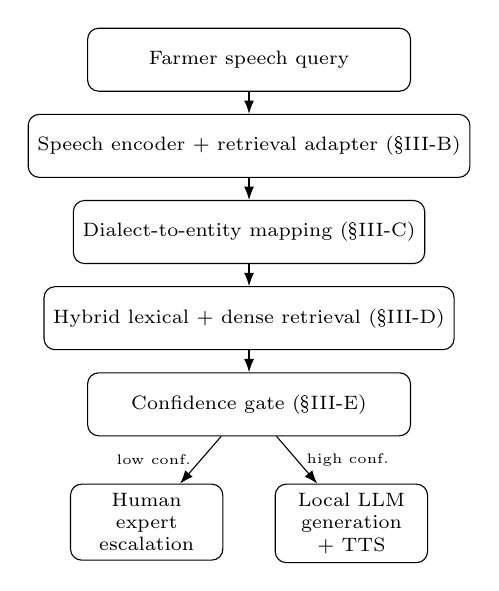
\begin{tikzpicture}[
  block/.style={rectangle, draw, rounded corners, align=center, minimum width=4.1cm, minimum height=0.8cm, font=\scriptsize},
  smallblock/.style={rectangle, draw, rounded corners, align=center, text width=1.7cm, font=\scriptsize},
  arr/.style={-Latex}
]
\node[block] (speech) {Farmer speech query};
\node[block, below=0.28cm of speech] (enc) {Speech encoder + retrieval adapter (\S III-B)};
\node[block, below=0.28cm of enc] (dial) {Dialect-to-entity mapping (\S III-C)};
\node[block, below=0.28cm of dial] (hyb) {Hybrid lexical + dense retrieval (\S III-D)};
\node[block, below=0.28cm of hyb] (conf) {Confidence gate (\S III-E)};
\node[smallblock, below=0.6cm of conf, xshift=-1.3cm] (esc) {Human expert escalation};
\node[smallblock, below=0.6cm of conf, xshift=1.3cm] (gen) {Local LLM generation + TTS};

\draw[arr] (speech) -- (enc);
\draw[arr] (enc) -- (dial);
\draw[arr] (dial) -- (hyb);
\draw[arr] (hyb) -- (conf);
\draw[arr] (conf) -- node[left,font=\tiny]{low conf.} (esc);
\draw[arr] (conf) -- node[right,font=\tiny]{high conf.} (gen);
\end{tikzpicture}
\caption{Proposed pipeline. All stages except one-time adapter training (\S III-F) run fully offline on consumer-grade hardware.}
\label{fig:architecture}
\end{figure}

\subsection{Speech-Native Retrieval Backbone}
Following SpeechRAG \cite{min2025speechrag} and Google's S2R \cite{google2025s2r}, the pipeline fine-tunes a lightweight adapter that projects representations from a pretrained speech encoder --- wav2vec 2.0 \cite{baevski2020wav2vec}, HuBERT \cite{hsu2021hubert}, or a multilingual encoder such as SeamlessM4T \cite{barrault2023seamlessm4t} where the target dialect lacks dedicated pretraining data --- into the embedding space of a frozen text retriever, extending the dense-retrieval formulation of Karpukhin et al. \cite{karpukhin2020dpr} to operate on speech rather than text queries. This adapter is the only component in the pipeline permitted to use cloud GPU resources, and only once, at training time (contribution 4); at inference time it runs locally alongside the rest of the pipeline. Unlike the evaluations reported for SpeechRAG and S2R, the adapter here is trained and evaluated with explicit attention to two conditions neither prior system tested: queries containing domain-critical rare entities (pesticide, pest, and disease names) and queries spoken in dialectal or code-mixed variants of the target language, motivated by evidence that both conditions independently degrade ASR transcription accuracy \cite{benchmarkingasr2026,dialectmatters2026} and are expected to compound when they co-occur, consistent with the ``textless NLP'' premise that representations optimized for transcription accuracy are not necessarily optimal for downstream retrieval \cite{spidr2025}.

\subsection{Dialect-to-Scientific-Entity Mapping Layer}
Retrieval collapses if a normalized speech embedding still fails to align with a document indexed under standardized nomenclature. The mapping layer addresses this by bootstrapping a dialect-term-to-scientific-entity lexicon from existing public resources --- agricultural knowledge graphs such as Crop GraphRAG \cite{wu2026cropgraphrag}, named-entity resources such as AgCNER \cite{yao2024agcner}, and standards-level ontologies such as EPPO \cite{kgeditorial2023} --- rather than through new dialect speech collection, consistent with contribution 2. This follows the same motivation as the soft-prompt-tuning approach of Liu et al. \cite{liu2025colloquialpest}, which showed that conventional classifiers degrade substantially on farmers' colloquial symptom descriptions, and the keyword-injection strategy used in the Bengali cross-lingual RAG case study \cite{hossain2026bengalirag}; both operate on written text, whereas the mapping layer proposed here is designed to operate on the speech-embedding representation produced in Section III-B, since that system's own future-work discussion identifies dialect-aware normalization of spoken queries as unresolved. Two integration strategies are considered: a post-ASR text-normalization path, retained only as a fallback because it reintroduces a transcription dependency for this one layer, and an embedding-space mapping path that aligns dialect-term speech embeddings directly against the retriever's embedding space, preferred because it requires no transcription step anywhere in the pipeline.

\subsection{Hybrid Retrieval Strategy}
Comparative retrieval studies show dense retrieval outperforming lexical retrieval on paraphrased queries with low lexical overlap, while lexical methods such as BM25 retain the advantage on exact, rare, domain-specific entities \cite{sultania2024hybridsearch} --- precisely the pesticide and disease name category this paper treats as safety-critical. The architecture therefore fuses lexical and dense signals rather than committing to either alone, so that a colloquial, paraphrased query and an exact rare-entity query are both served by the retrieval mode best suited to it. This choice is deliberately positioned against a naive ``speech embeddings beat keywords'' framing: since a purely dense speech-native retriever risks losing precisely the safety-critical query category to a simpler keyword baseline, hybrid retrieval is treated as the default backbone to be evaluated, not a strict either/or alternative to speech-native retrieval.

\subsection{Confidence-Gated Escalation}
Because an incorrect agricultural recommendation can damage a season's crop, the architecture inserts a confidence gate between retrieval and answer generation, following the case made for confidence-gated abstention in comparably high-stakes clinical and financial RAG deployments \cite{abstinence2025}. The gate combines closed-book signals (internal model confidence) and open-book signals (divergence between model behavior with and without retrieved context), following the taxonomy of Dependable RAG \cite{dependablerag2026}, rather than relying on a single score. This design choice is directly informed by a documented failure mode: naive entropy-based confidence signals have been shown to misfire in both directions, flagging correct, well-grounded answers as uncertain due to interactions between attention mechanisms and entropy computation \cite{intrygue2026}. Accordingly, the gate is treated as a component requiring empirical validation against labeled correct/incorrect examples (Section IV-E) rather than a mechanism assumed reliable by construction. Queries falling below the confidence threshold are escalated to a human expert rather than answered, mirroring the human-in-the-loop fallback already present in call-center-style deployments such as KrishokBondhu \cite{ameen2026krishokbondhu}.

\subsection{Offline Deployment Scoping}
All pipeline stages other than the one-time speech-retrieval adapter training (Section III-B) are required to run without a live network connection, on consumer-grade, GPU-constrained hardware. This mirrors the deployment pattern already demonstrated for text-only offline agricultural RAG systems such as A.A.H.A.R. \cite{dubey2025aahar} and the Bengali cross-lingual RAG case study \cite{hossain2026bengalirag}, and for a vision-modality offline system in rural Tigray \cite{tigray2025plantdisease}, and is bounded by reported feasibility figures for quantized on-device language models --- 2--3 tokens/second for 4-bit Llama-3 8B on a smartphone with at least 6 GB RAM, with 8-bit variants requiring a discrete GPU with at least 8 GB VRAM for comparable throughput \cite{compactllm2026}. Whether these figures still hold once a speech encoder, adapter, dialect-mapping layer, and confidence gate are added on top of the language model is treated as an open question (RQ3) evaluated in Section IV, not an assumption carried over from text-only systems.

\section{Experimental Protocol}

\subsection{Overview}
No experiments have yet been executed; this section specifies the protocol by which the architecture in Section III would be evaluated against RQ1--RQ4, so that the evaluation plan in Section V can be read as a set of falsifiable hypotheses rather than an assumed outcome.

\subsection{Query Dataset Construction}
The evaluation requires a query set stratified along two axes motivated in Sections I and III: standard-terminology versus dialectal/colloquial phrasing, and common versus domain-critical rare-entity queries (pesticide, pest, and disease names). Prior characterizations of real farmer helpline query volume and content \cite{godara2022querycount,godara2020sequentialpattern} inform the query distribution the dataset should approximate, so that the stratified test set is representative of actual query patterns rather than an artificially uniform sample. Where dedicated dialect speech resources exist, such as the RESPIN Chhattisgarhi corpus \cite{singh2023respin}, they are used directly; where the target dialect has no comparable resource, a small evaluation set is collected specifically for the rare-entity and dialectal strata, consistent with the constraint that no large new dialect speech corpus is collected for training (Section III-C).

\subsection{Baselines and Conditions}
Four retrieval conditions are compared under identical query sets, isolating the specific comparisons RQ1 and RQ4 require:

\begin{enumerate}
    \item \textbf{ASR-cascaded retrieval} --- a Whisper-based \cite{radford2023whisper} transcription step followed by text retrieval, representing the dominant existing design pattern (Farmer.Chat, KrishokBondhu, A.A.H.A.R., Krishi Sathi).
    \item \textbf{Keyword-only (lexical) retrieval} --- BM25 over ASR transcripts, isolating lexical retrieval performance in the presence of transcription error.
    \item \textbf{Dense semantic retrieval} --- text-embedding retrieval following the dense passage retrieval formulation \cite{karpukhin2020dpr}, applied both to ASR transcripts and, where applicable, to speech-native embeddings from Section III-B.
    \item \textbf{Hybrid retrieval} --- the fused lexical-dense condition of Section III-D, evaluated both with and without the dialect-to-entity mapping layer of Section III-C, isolating the mapping layer's contribution (RQ2).
\end{enumerate}

All conditions retrieve from the same underlying knowledge base, constructed following the retrieval-augmented generation formulation of Lewis et al. \cite{lewis2020rag}, so that differences in measured accuracy are attributable to the retrieval mechanism rather than to differences in the underlying corpus.

\subsection{Evaluation Metrics}
Retrieval quality is measured with standard recall@$k$ and mean reciprocal rank, reported separately for the standard-terminology and dialectal/rare-entity strata rather than as a single aggregate figure, following the rationale that aggregate metrics can mask exactly the failure mode this paper targets --- the same rationale underlying the agriculture-weighted WER metric proposed for ASR evaluation \cite{benchmarkingasr2026}. End-to-end latency is measured from spoken query to delivered answer on the target consumer-hardware configuration (Section IV-F). Confidence-gate quality is measured separately from retrieval quality, via calibration error and via abstention precision/recall against a labeled set of known-correct and known-incorrect answers, directly addressing the INTRYGUE-documented risk that confidence signals can misfire in both directions \cite{intrygue2026}.

\subsection{Confidence Gate Validation Protocol}
Because a miscalibrated gate can be worse than no gate at all \cite{intrygue2026}, the gate is validated on a held-out labeled set before being used to report any end-to-end system result: candidate confidence signals (closed-book and open-book, per \cite{dependablerag2026}) are scored against ground-truth correctness labels, and a signal or combination of signals is adopted for the full pipeline only if it exceeds a pre-registered calibration threshold on this held-out set.

\subsection{Hardware Target}
All inference-time components (Sections III-B through III-E) are benchmarked on a single, explicitly stated consumer-hardware configuration --- a GPU-constrained laptop or mini-PC class device, consistent with the RAM/VRAM figures in \cite{compactllm2026} --- rather than left as an unspecified ``consumer-grade'' claim, so that the latency and accuracy figures reported in Section V are reproducible against a fixed target.

\section{Evaluation Plan and Expected Outcomes}

As the protocol in Section IV has not yet been executed, this section states, for each research question, the comparison that would answer it and the pattern of results that would confirm or disconfirm the corresponding hypothesis --- not observed data.

\subsection{RQ1 --- Speech-Native Retrieval Under Dialect and Rare-Entity Conditions}
\textbf{Hypothesis:} speech-native retrieval (Section III-B) matches or exceeds ASR-cascaded retrieval in aggregate, consistent with prior results for SpeechRAG and S2R \cite{min2025speechrag,google2025s2r}, but the size of that advantage is expected to \emph{grow} on the dialectal and rare-entity strata specifically, since those are exactly the conditions under which ASR transcription error concentrates \cite{benchmarkingasr2026,dialectmatters2026}. \textbf{Disconfirming pattern:} if the speech-native advantage shrinks or reverses on the dialectal/rare-entity strata relative to the standard-terminology stratum, this would indicate the adapter itself fails to generalize to dialect variation, motivating dialect-specific adapter fine-tuning as future work rather than confirming RQ1 as stated.

\subsection{RQ2 --- Dialect-to-Entity Mapping Contribution}
\textbf{Hypothesis:} hybrid retrieval with the mapping layer (Section III-C) outperforms hybrid retrieval without it specifically on the dialectal/colloquial query stratum, with little or no difference on the standard-terminology stratum, isolating the mapping layer's contribution to exactly the queries it targets. \textbf{Disconfirming pattern:} a uniform improvement across both strata would suggest the mapping layer is acting as a general retrieval-quality improvement rather than a dialect-specific one, which would still be a positive result but would not confirm RQ2 as a dialect-targeted claim.

\subsection{RQ3 --- Offline Feasibility on Consumer Hardware}
\textbf{Hypothesis:} the full pipeline meets a pre-specified latency budget (informed by the sub-2-second to sub-20-second range reported for text-only offline agricultural systems \cite{dubey2025aahar,hossain2026bengalirag}, adjusted upward for the added speech and mapping components) on the hardware target specified in Section IV-F, without a significant accuracy regression relative to a cloud-hosted configuration of the same pipeline. \textbf{Disconfirming pattern:} if latency exceeds the budget or accuracy regresses substantially under quantization, this would indicate the current architecture requires either further compression or a revised hardware target, directly answering RQ3 in the negative rather than leaving it unresolved.

\subsection{RQ4 --- Hybrid Retrieval with Dialect Mapping vs.\ Either Alone}
\textbf{Hypothesis:} hybrid retrieval combined with dialect mapping outperforms lexical-only and dense-only retrieval individually on the rare-entity stratum, where prior comparative work predicts lexical and dense methods trade off \cite{sultania2024hybridsearch}, confirming that neither method alone is sufficient once dialect variation and rare entities co-occur. \textbf{Disconfirming pattern:} if one retrieval mode alone matches hybrid performance even on the rare-entity stratum, this would indicate the hybrid fusion adds complexity without a corresponding accuracy benefit for this query population.

\subsection{Threats to Validity}
The evaluation plan above depends on dialect-stratified query data whose scale is inherently limited by the absence of large existing dialect speech resources for the target dialect (Section IV-B), which constrains statistical power on exactly the strata RQ1 and RQ2 depend on; this limitation, and mitigations such as bootstrapped or synthetic dialectal query augmentation, are discussed further in Section VII.

\section{Prototype Implementation and Preliminary Measurements}

\subsection{Scope and Purpose of This Section}
Sections III--V describe an architecture and a protocol for evaluating it, and state explicitly that the protocol had not been executed. Since that text was written, a best-effort, genuinely runnable software prototype of the architecture in Section III has been built and exercised end to end, and this section reports the real, measured numbers that prototype produces. This is not the same thing as executing the Section IV protocol: the prototype runs on small, hand-curated, demo-scale data rather than the dialect-stratified corpus Section IV-B calls for, and --- because no recorded speech corpus for the target dialect exists, which remains this paper's central open problem --- every audio-involving measurement below uses \texttt{espeak-ng} text-to-speech synthesis of query text rather than native dialect speech. The results in this section should therefore be read as an engineering stress-test of the mechanism proposed in Section III: evidence that each component runs, composes, and behaves sensibly, not as an answer to RQ1--RQ4 as posed. Section V's hypotheses remain open; Section VI-G states precisely what this prototype does and does not change about that.

\subsection{Prototype System and Demo Data}
The prototype implements all four pipeline stages of Fig.~\ref{fig:architecture}: a hybrid BM25 + dense retriever (Reciprocal Rank Fusion, $k=60$) over a 42-passage hand-authored agricultural knowledge base spanning common and domain-critical-rare pest, disease, and pesticide entries; a 29-entry dialect-to-entity lexicon bootstrapped, per the contribution-2 constraint, from generally known North/Central-Indian farmer-extension terminology rather than a domain-expert-reviewed or public-KG-sourced resource --- a demo-scale stand-in for the resource contribution 2 specifies, not that resource itself; a speech-native retrieval adapter (frozen wav2vec2 \cite{baevski2020wav2vec} encoder plus a small trained projection head, following \cite{min2025speechrag,google2025s2r}) trained with an in-batch InfoNCE contrastive objective; an ASR-cascaded baseline using \texttt{faster-whisper} ``tiny'' \cite{radford2023whisper}; and a confidence gate combining a closed-book retrieval-margin signal with an open-book lexical-grounding-overlap signal, per the taxonomy of \cite{dependablerag2026}. Generation uses Qwen2.5-0.5B-Instruct in fp16, falling back to a deterministic template when the LLM is unavailable. All measurements below were run on a single NVIDIA RTX 3050 Laptop GPU (6~GB VRAM), stating a concrete hardware target as Section IV-F requires. Evaluation uses 50 queries stratified 2$\times$2 over standard/dialectal phrasing and common/domain-critical-rare entities, matching Section IV-B's stratification design.

\subsection{Retrieval Comparison}
Table~\ref{tab:retrieval} reports recall@1, by query stratum, for six retrieval conditions. Dialect mapping is the single largest lever measured: every condition without it scores at or near zero recall@1 on both dialectal strata, while adding it (condition 4) raises dialectal recall@1 to 0.615 --- a real, clean, demo-scale confirmation of the RQ2/RQ4 premise that a mapping layer is specifically what unlocks dialectal queries, though the 42-passage KB used here has fairly distinct inter-passage vocabulary, and the same experiment on a larger, messier knowledge base would need to be re-run before trusting this exact figure. The ASR-cascaded baseline (condition 5) is badly degraded by dialectal queries (0.000 recall@1 on both dialectal strata) and, notably, underperforms text-only hybrid retrieval even on standard-phrasing queries (0.583 vs.\ 0.917 on standard/common), because Whisper ``tiny'' mistranscribes even the synthetic English-voice audio substantially; this is consistent with the ASR-error concentration reported by \cite{benchmarkingasr2026,dialectmatters2026}, but should be read as a property of this specific small model and synthetic-audio pipeline, not a general claim about Whisper. (A same-day re-run of this evaluation reproduced every other cell in this table exactly and this condition's dialectal/common cell specifically at 0.000 rather than an earlier 0.077 --- one query's transcription flipping between correct and incorrect --- consistent with the run-to-run non-determinism of \texttt{faster-whisper} on GPU already discussed in \texttt{implementation/README.md}; the qualitative finding is unchanged.) The trained speech-native adapter (condition 6) scores 0.020 recall@1 overall on this held-out eval set --- effectively chance for a 42-way retrieval problem --- despite demonstrably learning a real retrieval signal on its own training distribution (Section VI-D) --- a genuine, and informative, negative result rather than an implementation defect.

\begin{table*}[t]
\caption{Recall@1 by retrieval condition and query stratum (prototype, $n{=}50$ demo eval queries; see Section VI-A for scope caveats)}
\centering
\footnotesize
\begin{tabular}{@{}lccccc@{}}
\toprule
\textbf{Condition} & \textbf{All} & \textbf{Std./Common} & \textbf{Std./Rare} & \textbf{Dial./Common} & \textbf{Dial./Rare} \\
\midrule
1. Keyword only (BM25)                    & 0.500 & 0.917 & 1.000 & 0.077 & 0.077 \\
2. Dense only                              & 0.400 & 0.833 & 0.833 & 0.000 & 0.000 \\
3. Hybrid, no dialect mapping              & 0.460 & 0.917 & 1.000 & 0.000 & 0.000 \\
4. Hybrid + dialect mapping                & \textbf{0.780} & 0.917 & 1.000 & \textbf{0.615} & \textbf{0.615} \\
5. ASR cascade + hybrid + dialect mapping  & 0.380 & 0.583 & 1.000 & 0.000 & 0.000 \\
6. Speech-native adapter, no dialect mapping & 0.020 & 0.000 & 0.000 & 0.000 & 0.077 \\
\bottomrule
\end{tabular}
\label{tab:retrieval}
\end{table*}

\subsection{Speech-Native Adapter: Mechanism Works, Generalization Does Not}
Trained for 100 epochs (fixed seed, $\sim$20~s wall time) with an in-batch InfoNCE contrastive loss on 108 auto-generated English template sentences, the adapter reaches 61.1\% top-1 passage retrieval accuracy on its own 18-example held-out validation split --- roughly 26$\times$ the 2.4\% chance level for this 42-way retrieval problem, and a real, positive demonstration that the frozen-speech-encoder-plus-small-adapter mechanism of \cite{min2025speechrag,google2025s2r} works end to end without any transcription step. On \texttt{eval\_queries.jsonl}'s full natural-language symptom descriptions and romanized dialectal queries --- a materially different phrasing distribution from the short templates it trained on --- recall@1 falls to 0.020 overall (Table~\ref{tab:retrieval}, condition 6), effectively at chance. This generalization gap is exactly the kind of result RQ1 anticipates as an open question rather than assumes resolved: the mechanism transfers, a small synthetic training signal does not, and dialect-speech generalization specifically remains untested by this prototype, since no dialect speech data exists to test it on.

\subsection{Confidence Gate Validation}
Following the Section IV-E protocol, the gate was validated on 50 labeled examples (39 correct / 11 incorrect; unconditional accuracy 0.780) before being credited with any end-to-end result. Table~\ref{tab:gate} shows the threshold sweep: at threshold 0.5, the gate answers 32\% of queries at 0.875 accuracy (vs.\ the 0.780 always-answer baseline) while escalating 81.8\% of the actually-wrong answers in the set. This clears the minimal bar a confidence gate must clear. Validation also surfaced a real limitation, exactly the kind \cite{intrygue2026} warns naive confidence signals can hide: the open-book grounding-overlap signal varies only from 0.868 to 0.937 across every example in this run, correct or not, because the templated answers used to build this labeled set quote their own top-1 passage verbatim --- so the answer is ``grounded'' by construction even when that passage is wrong. Almost all of the gate's discriminative power in this run therefore comes from the closed-book retrieval-margin signal alone, not the closed-book/open-book combination the design in Section III-E intended (Expected Calibration Error over 5 bins: 0.291). This is the validation step named in Section IV-E doing precisely what it is for: catching, before deployment, a signal that looks reasonable in aggregate but is silently carried by only one of its inputs. A production version of the gate would need this signal re-validated against non-template-quoting LLM answers, where grounding overlap can actually diverge from correctness.

\begin{table}[t]
\caption{Confidence gate threshold sweep (prototype, $n{=}50$ labeled examples)}
\begin{center}
\begin{tabular}{@{}ccccc@{}}
\toprule
\textbf{Thresh.} & \textbf{Coverage} & \textbf{Acc. if ans.} & \textbf{Esc. prec.} & \textbf{Esc. recall} \\
\midrule
0.4 & 1.000 & 0.780 & n/a & 0.000 \\
0.5 & 0.320 & 0.875 & 0.265 & 0.818 \\
0.6 & 0.000 & n/a & 0.220 & 1.000 \\
\bottomrule
\end{tabular}
\end{center}
\label{tab:gate}
\end{table}

\subsection{Offline Latency and Memory (RQ3)}
Table~\ref{tab:latency} reports steady-state per-stage latency on the RTX 3050 Laptop target. Dialect mapping, hybrid retrieval, and the confidence gate are each sub-10~ms and effectively free next to generation; LLM generation dominates end-to-end latency at $\sim$1.3~s mean for a 120-token-capped response. Peak VRAM with every model loaded simultaneously --- dense retriever, Whisper tiny, wav2vec2 plus adapter, and the fp16 LLM --- measured 1.54~GB, comfortably inside the 6~GB budget with $\sim$4.5~GB headroom. This lands in roughly the same sub-2-second ballpark reported for a comparable offline agricultural LLM system on comparable hardware \cite{dubey2025aahar}, which is consistent with, though not proof of, RQ3's premise holding once the speech, dialect-mapping, and confidence-gating layers are stacked on top of generation --- for this demo-scale, 42-passage KB. The LLM here runs in fp16, not INT4/INT8-quantized, so the throughput figures reported for quantized on-device models \cite{compactllm2026} remain uncompared against a quantized version of this exact pipeline; retrieval latency over a production-scale KB (thousands of passages) also should not be extrapolated linearly from this 42-passage result.

\begin{table}[t]
\caption{Steady-state per-stage latency, text-query path (prototype, RTX 3050 Laptop 6GB, $n{=}20$)}
\begin{center}
\begin{tabular}{@{}lrr@{}}
\toprule
\textbf{Stage} & \textbf{Mean} & \textbf{p95} \\
\midrule
Dialect mapping                     & 0.1~ms   & 0.6~ms \\
Hybrid search (BM25+dense+fusion)   & 3.8~ms   & 4.3~ms \\
Confidence gate scoring             & 0.0~ms   & 0.1~ms \\
LLM generation ($\le$120 tok)       & 1282.5~ms & 1476.4~ms \\
\bottomrule
\end{tabular}
\end{center}
\label{tab:latency}
\end{table}

\subsection{What This Prototype Does and Does Not Establish}
Taken together, this prototype demonstrates that the architecture of Section III is buildable, that its four components compose into a working end-to-end pipeline (24 passing tests across retrieval, dialect mapping, the confidence gate, and full-pipeline smoke tests), and that on demo-scale data the mechanism behaves in the direction the paper's hypotheses predict for dialect mapping (RQ2) and offline latency (RQ3), while surfacing two genuine open problems --- speech-native retrieval's generalization gap (RQ1) and the confidence gate's open-book signal weakness --- that a purely architectural proposal could not have discovered. It does not establish that these results hold on real dialect speech, at production knowledge-base scale, or under a quantized deployment target, and it does not substitute for the dialect-stratified evaluation Section IV-B specifies on the target dialect, since the underlying speech data for that evaluation still does not exist. Section V's hypotheses are therefore still open exactly as stated; this section adds a real, if small and demo-scale, existence proof that the mechanism designed to test them runs.

\section{Conclusion}

This paper has argued that no existing agricultural advisory system combines speech-native retrieval, dialect-to-scientific-entity mapping, confidence-gated escalation, and fully offline operation, despite each being independently established: speech-native retrieval has been shown to match or exceed ASR-cascaded retrieval in general-purpose settings \cite{min2025speechrag,google2025s2r}; colloquial-to-formal entity mapping has been shown to be necessary and tractable in text \cite{liu2025colloquialpest,hossain2026bengalirag}; confidence-gated abstention has been argued for in other high-stakes RAG domains \cite{abstinence2025}; and offline deployment has been demonstrated for text-based agricultural RAG specifically \cite{dubey2025aahar,hossain2026bengalirag}. Section III integrates these four components into a single pipeline, Section IV and Section V specify how each of RQ1--RQ4 would be tested and what pattern of results would confirm or disconfirm each hypothesis, and Section VI reports real measurements from a runnable prototype of that pipeline on demo-scale data.

The principal limitation of the present paper is that its central research questions remain empirically open on the target dialect: the prototype reported in Section VI demonstrates that the architecture of Section III is buildable and behaves, on demo-scale data, in the direction the paper's hypotheses predict for dialect mapping and offline latency --- while also surfacing two genuine unresolved problems, the speech-native adapter's failure to generalize past its training distribution and a confidence-gate signal that validation revealed was less discriminative than intended --- but no component has yet been evaluated on real target-dialect speech, because that corpus does not exist, and the hypotheses in Section V are therefore still predictions to be tested rather than reported findings. Committing to a falsifiable protocol (Section IV) before running experiments, and then reporting the prototype's negative and partial results in Section VI alongside its positive ones, is intended to guard against the kind of confirmation-driven evaluation that a system built and evaluated by the same process would otherwise risk, particularly for the confidence-gating component, where \cite{intrygue2026} shows that superficially reasonable confidence signals can fail silently --- a failure mode Section VI-E shows this prototype actually exhibiting, not merely warns against.

Future work is therefore the direct execution of Section IV on real data: collection or acquisition of the dialect-stratified evaluation set described in Section IV-B for the target dialect, re-training and re-evaluating the speech-native adapter and dialect-mapping layer on that data rather than the demo corpus and synthetic TTS audio used in Section VI, implementation of the embedding-space dialect-mapping path so that dialect mapping composes with speech-native retrieval rather than only the post-ASR text path evaluated here, re-validation of the confidence gate's open-book signal against non-template-quoting LLM answers, and quantization of the local LLM to test the offline latency figures of Section VI-F under the RQ3-relevant deployment target rather than fp16. Beyond executing this protocol, two extensions follow naturally from the synthesis discussion in Section II: first, extending the dialect-to-entity mapping layer beyond the single target dialect evaluated here, toward the many Indian dialects that, like the one targeted in this paper, presently have no dedicated speech or mapping resource \cite{dialectmatters2026,singh2023respin}; and second, examining whether the confidence-gating and offline-deployment components generalize to other high-stakes, low-connectivity domains --- clinical and financial advisory --- where confidence-gated RAG has been argued for but not, to this paper's knowledge, combined with speech-native retrieval either \cite{dependablerag2026,abstinence2025}.


% \subsection{Abbreviations and Acronyms}\label{AA}
% Define abbreviations and acronyms the first time they are used in the text, 


% \subsection{Units}
% \begin{itemize}
% \item Use either SI
% \item Avoid 
% \end{itemize}

% \subsection{Equations}
% Number 
% \begin{equation}
% a+b=\gamma\label{eq}
% \end{equation}


% \subsection{Figures and Tables}
% \paragraph{Po 
% ``Fig.~\ref{fig}'', even at the beginning of a sentence.

% \begin{table}[htbp]
% \caption{Table Type Styles}
% \begin{center}
% \begin{tabular}{|c|c|c|c|}
% \hline
% \textbf{Table}&\multicolumn{3}{|c|}{\textbf{Table Column Head}} \\
% \cline{2-4} 
% \textbf{Head} & \textbf{\textit{Table column subhead}}& \textbf{\textit{Subhead}}& \textbf{\textit{Subhead}} \\
% \hline
% copy& More table copy$^{\mathrm{a}}$& &  \\
% \hline
% \multicolumn{4}{l}{$^{\mathrm{a}}$Sample of a Table footnote.}
% \end{tabular}
% \label{tab1}
% \end{center}
% \end{table}

% \begin{figure}[htbp]
% \centerline{\includegraphics{fig1.png}}
% \caption{Example of a figure caption.}
% \label{fig}
% \end{figure}

% Figure Labels: Use 8 point Times New Roman for Figure labels. Use words 
% rather than symbols or abbreviations when writing Figure axis labels to 
% avoid confusing the reader. As an example, write the quantity 
% ``Magnetization'', or ``Magnetization, M'', not just ``M''. If including 
% units in the label, present them within parentheses. Do not label axes only 
% with units. In the example, write ``Magnetization (A/m)'' or ``Magnetization 
% \{A[m(1)]\}'', not just ``A/m''. Do not label axes with a ratio of 
% quantities and units. For example, write ``Temperature (K)'', not 
% ``Temperature/K''.


% \section*{Acknowledgment}

% The preferred spelling of the word ``acknowledgment'' in America is without 
% an ``e'' after the ``g''. Avoid the stilted expression ``one of us (R. B. 
% G.) thanks $\ldots$''. Instead, try ``R. B. G. thanks$\ldots$''. Put sponsor 
% acknowledgments in the unnumbered footnote on the first page.

\bibliographystyle{IEEEtran}
\bibliography{reference}

\end{document}
